\section{Hybrid modal ROM from static solves}\label{sec:vf-hyrom}

\subsection*{Concept and purpose}

\citet{yang2019hybrid} train a modal reduced model of a geometrically nonlinear structure from \emph{static} solves of the full-order model (implicit condensation) and then use it for forced transient response. The full nonlinear internal force is replaced by a linear part plus a nonlinear modal force that is a polynomial in the modal coordinates, and the coefficients are fitted by least squares to static data. The study tests two structures of different character: a cantilever plate with a hole, whose free edge lets in-plane motion occur, and a hinged shallow cylindrical panel, whose edges are fixed in space. The test of the method is not the static fit, which is easy, but whether the model predicts a strongly nonlinear forced transient and, as an added check that a transient can hide, the free-vibration backbone.

The finite element models use \anchor{fea_engine.elements.Shell4Director} and \anchor{fea_engine.elements.Shell4MITC}; the reduced model is the polynomial modal model of \rom{} (\anchor{rom_engine.PolynomialModalROM}) with the Newmark integrator for reduced models and the Koiter--Newton static solver of \fea{} for the panel.

\subsection*{Mathematics as implemented}

The semi-discrete full-order model with $n$ free degrees of freedom is
\begin{equation}\label{eq:hy-fom}
\mathbf M\ddot{\mathbf u}+\mathbf C\dot{\mathbf u}+\mathbf f_{\rm int}(\mathbf u)=\mathbf f_{\rm ext}(t),
\end{equation}
with the linear tangent stiffness $\mathbf K=\partial\mathbf f_{\rm int}/\partial\mathbf u|_{\mathbf 0}$ and mass-normalised modes $\mathbf V^{T}\mathbf M\mathbf V=\mathbf I$, $\mathbf K\boldsymbol\phi_r=\lambda_r\mathbf M\boldsymbol\phi_r$, $\lambda_r=(2\pi f_r)^2$. Projecting $\mathbf u\approx\mathbf V\mathbf q$ gives the $N$-degree-of-freedom model
\begin{equation}\label{eq:hy-rom}
\ddot{\mathbf q}+\mathbf C_r\dot{\mathbf q}+\boldsymbol\Lambda\mathbf q+\mathbf F_{\rm nl}(\mathbf q)=\mathbf V^{T}\mathbf f_{\rm ext}(t),\qquad\boldsymbol\Lambda=\operatorname{diag}(\lambda_r).
\end{equation}

\emph{Identification.} For training sample $i$ a modal force $\hat{\mathbf f}_i$ is drawn, the physical load is $\mathbf F_i=\mathbf M\mathbf V\hat{\mathbf f}_i$ (so $\mathbf V^{T}\mathbf F_i=\hat{\mathbf f}_i$ exactly), and the nonlinear static problem $\mathbf f_{\rm int}(\mathbf u_i)=\mathbf F_i$ is solved. Projection gives
\begin{equation}\label{eq:hy-id}
\mathbf q_i^{\rm nl}=\mathbf V^{T}\mathbf M\mathbf u_i,\qquad\mathbf F_{{\rm nl},i}=\hat{\mathbf f}_i-\boldsymbol\Lambda\mathbf q_i^{\rm nl},
\end{equation}
and each component is fitted by ordinary least squares to the quadratic-plus-cubic form
\begin{equation}\label{eq:hy-nash}
F_{{\rm nl},r}(\mathbf q)=\sum_{i\le j}B_r(i,j)\,q_iq_j+\sum_{i\le j\le k}A_r(i,j,k)\,q_iq_jq_k,
\end{equation}
which has $N(N+1)/2+N(N+1)(N+2)/6$ terms (7 for $N=2$, 83 for $N=6$); the number of samples is $\max(\lceil1.3\,n_{\rm terms}\rceil,15)$ or more.

\emph{Training loads.} The target peak displacement of mode $r$ is drawn by optimal Latin-hypercube sampling in a range of $a_r$ thicknesses, $Q^{\max}_r=a_rh$, and the modal force follows as $\hat f_r=(Q_r^{\max}/\phi_r^{\max})\lambda_r$. The ranges are signed (push and pull) because the transient swings through both signs.

\emph{Time integration.} Newmark-$\beta$ ($\beta=\tfrac14$, $\gamma=\tfrac12$) with the nonlinear force treated implicitly, by \texttt{newton} (Newton on the reduced residual with the polynomial Jacobian), \texttt{fixed\_point} (four Picard sweeps; it matches \texttt{newton} to printed precision at the time steps used) or \texttt{sign\_deviation} (the predictor--corrector of \citet{he2023mfsnlrom}, Eq.~32). The last applies $\operatorname{sign}(\ddot q)\,[F_{\rm nl}(t{+}\Delta t)-F_{\rm nl}(t)]$; for modes with negative acceleration this reverses the correction, the error propagation is $2\mathbf I-\mathbf A$ instead of $\mathbf A$ with $\mathbf A=-\mathbf J_{\rm nl}\mathbf K_{\rm eff}^{-1}$, and it diverges on the panel for every mode set, so it is not used.

\emph{Metrics.} The transient error is
\begin{equation}\label{eq:hy-err}
\varepsilon=\frac{\max_t|w_{\rm ROM}(t)-w_{\rm FOM}(t)|}{\max_t|w_{\rm FOM}(t)|}.
\end{equation}
For the panel a projection baseline is also reported: the full-order history projected on the retained modes and reconstructed, the truncation-only floor of any model of that size. The backbone test releases mode~1 from a static state, oscillates undamped and measures the frequency against the linear one, giving $f/f_{\rm lin}$ against amplitude; agreement of the backbone shows that $\mathbf F_{\rm nl}$ is right \emph{dynamically}, not only statically.

\subsection*{Geometry and mesh}

Case~1 is a cantilever plate of aluminium, $1\times0.2\times0.01$~m, with a hole of radius $0.02$~m at mid-length, clamped at one end (7 nodes) and loaded by a 500~N, 2.5~Hz point force at the midpoint of the free end (\Cref{fig:vf-hy-mesh1}). The mesh has 204 nodes, 168 elements and 1224 degrees of freedom (the publication's has 2394). Case~2 is a shallow cylindrical panel of $R=2540$~mm, $L=508$~mm, $t=12.5$~mm and half-angle $0.1$~rad, with $E=3102.75$~MPa, $\nu=0.3$ and $\rho=5\times10^{-7}$~kg/mm$^3$, hinged on all four edges (translations fixed, rotations free) and loaded at the crown by 5000~N at 2.5~Hz (\Cref{fig:vf-hy-geom2}). The package has no curved-shell mesher, so a structured $10\times10$ grid in $(x,\theta)$ is mapped onto the cylinder (100 elements, 121 nodes, 726 degrees of freedom), and the crown load is spread over a $3\times3$ patch of nodes because a single-node load on this coarse mesh dimples locally too early.

\begin{figure}[tbp]
\centering
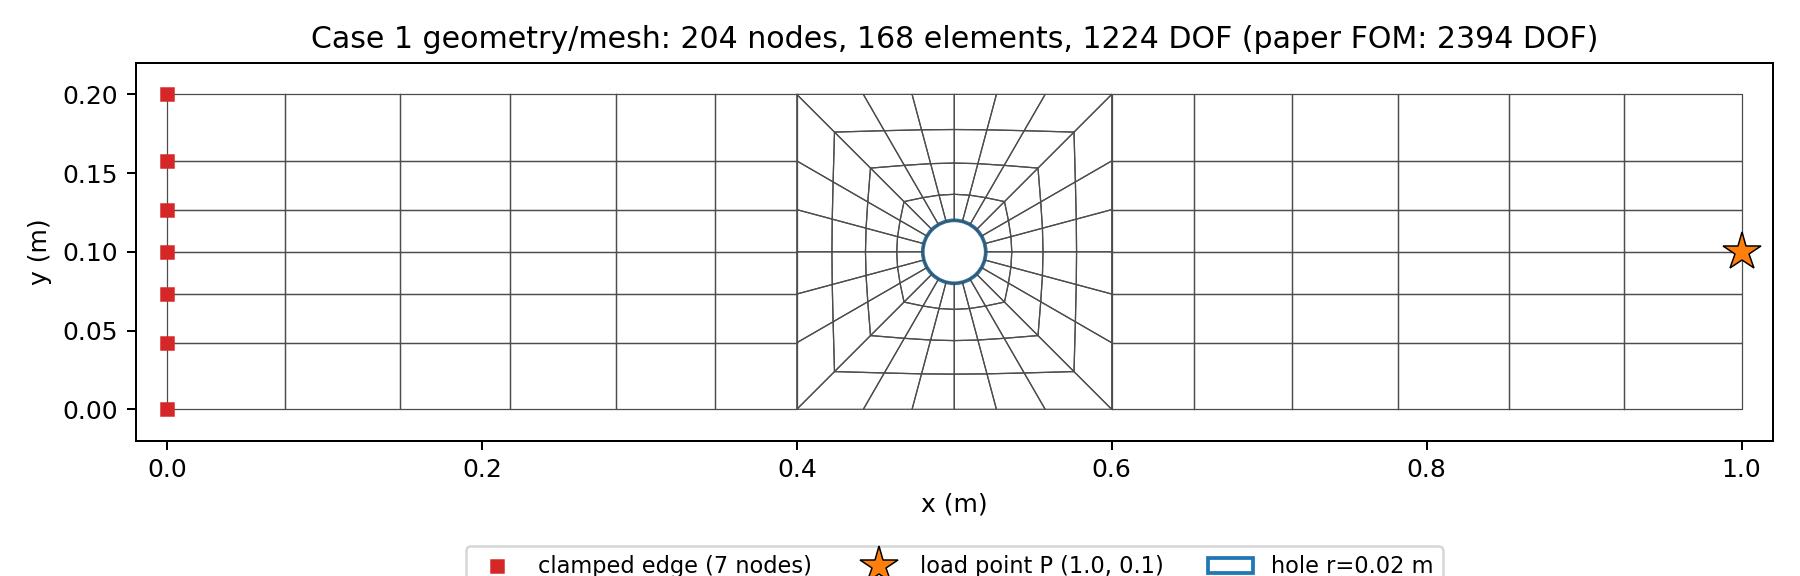
\includegraphics[width=0.8\linewidth]{figures/ch14r/hy_c1_mesh.png}
\caption{Case 1: plate with a hole. Mesh with 204 nodes and 168 elements (1224 degrees of freedom), clamped edge (red squares), load point (star) and the hole.}\label{fig:vf-hy-mesh1}
\end{figure}

\begin{figure}[tbp]
\centering
\includegraphics[width=0.95\linewidth]{figures/ch14_geom_hyrom.pdf}
\caption{Case 2: shallow cylindrical panel, drawn from the dimensions of the report. (a) The $10\times10$ mesh on the cylinder, hinged edge nodes, free nodes and the $3\times3$ crown load patch. (b) Section through the crown line.}\label{fig:vf-hy-geom2}
\end{figure}

\begin{table}[tbp]
\centering\footnotesize
\caption{Set-up of the two cases.}\label{tab:vf-hy-setup}
\begin{tabularx}{\linewidth}{@{}>{\raggedright\arraybackslash}p{3.0cm} >{\raggedright\arraybackslash}X >{\raggedright\arraybackslash}X@{}}
\toprule
Item & Case 1: plate with hole & Case 2: cylindrical panel\\
\midrule
Structure & cantilever $1\times0.2\times0.01$ m, hole $r=0.02$ m, aluminium & hinged panel $R=2540$, $L=508$, $t=12.5$ mm\\
Load & 500 N point load, 2.5 Hz & 5000 N crown load, 2.5 Hz\\
Size (this work / publication) & 1224 / 2394 dofs & 726 dofs\\
Training & 15 OLHS samples, signed ranges $q_1\in[-0.25,0.25]$, $q_2\in[-0.008,0.008]$; incremental Newton in 20 steps & 15 to 101 samples by mode set; Koiter--Newton ($\approx41$ s each)\\
Mode choice & modes 1, 2 & by projection of the load: 1, 6, 5, 9, 17, 16 (set sizes 2, 2, 3, 4, 6 as published, not the same hand-picked modes)\\
Time step & $\Delta t=0.005$ s, 200 steps & as in the publication\\
\bottomrule
\end{tabularx}
\end{table}

\subsection*{Results: verification of the full-order model}

\emph{Modes of case 1.} The four lowest frequencies are 8.35, 52.45, 81.60 and 150.49~Hz against 8.33, 51.98, 79.38 and 146.20~Hz in the publication, differences of $0.3$, $0.9$, $2.8$ and $2.9\,\%$ (\Cref{fig:vf-hy-modal}). The growth of the error with the mode number is plausibly the coarser mesh, which was not tested. For case~2 the modes 1 to 8 are 5.93, 9.63, 10.49, 15.40, 19.91, 20.41, 25.40 and 25.62~Hz; the publication gives no frequency table.

\begin{figure}[tbp]
\centering
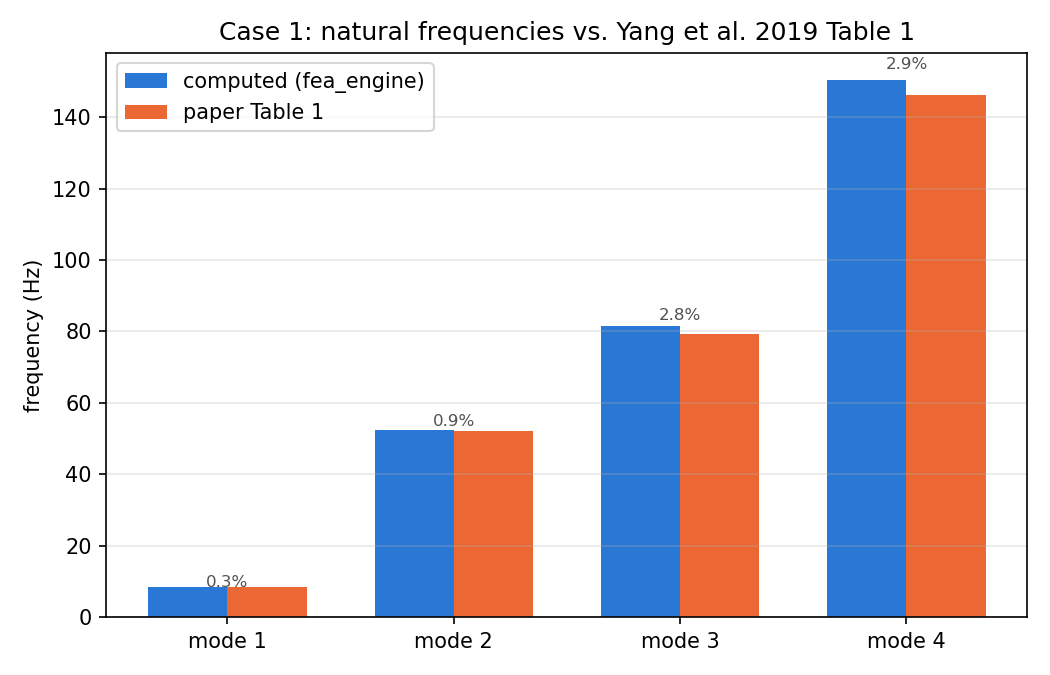
\includegraphics[width=0.6\linewidth]{figures/ch14r/hy_c1_modal.png}
\caption{Case 1: natural frequencies against the publication's Table~1.}\label{fig:vf-hy-modal}
\end{figure}

\emph{The element's geometric nonlinearity.} A first version of the case-1 model gave a nearly linear transient. The cause was the element, not the integrator: tested on a clamped strip with a tip load against the exact elastica, the shell element with a ``moderate'' curvature measure gave a tip-deflection ratio of $1.0005$ where the elastica gives $0.8725$, i.e.\ no stiffening at all. With the Green--Lagrange curvature measure of \texttt{Shell4Director} the ratio is $0.8729$ (\Cref{fig:vf-hy-elastica}). The narrow strips follow the elastica in stiffening and tip foreshortening; the plate-width strip deviates in stiffening and tip rotation, and the narrow strip at 40 elements diverges at the first load step, a separate robustness issue that remains open. The change moves the panel results by at most $0.15\,\%$ in displacement.

\begin{figure}[tbp]
\centering
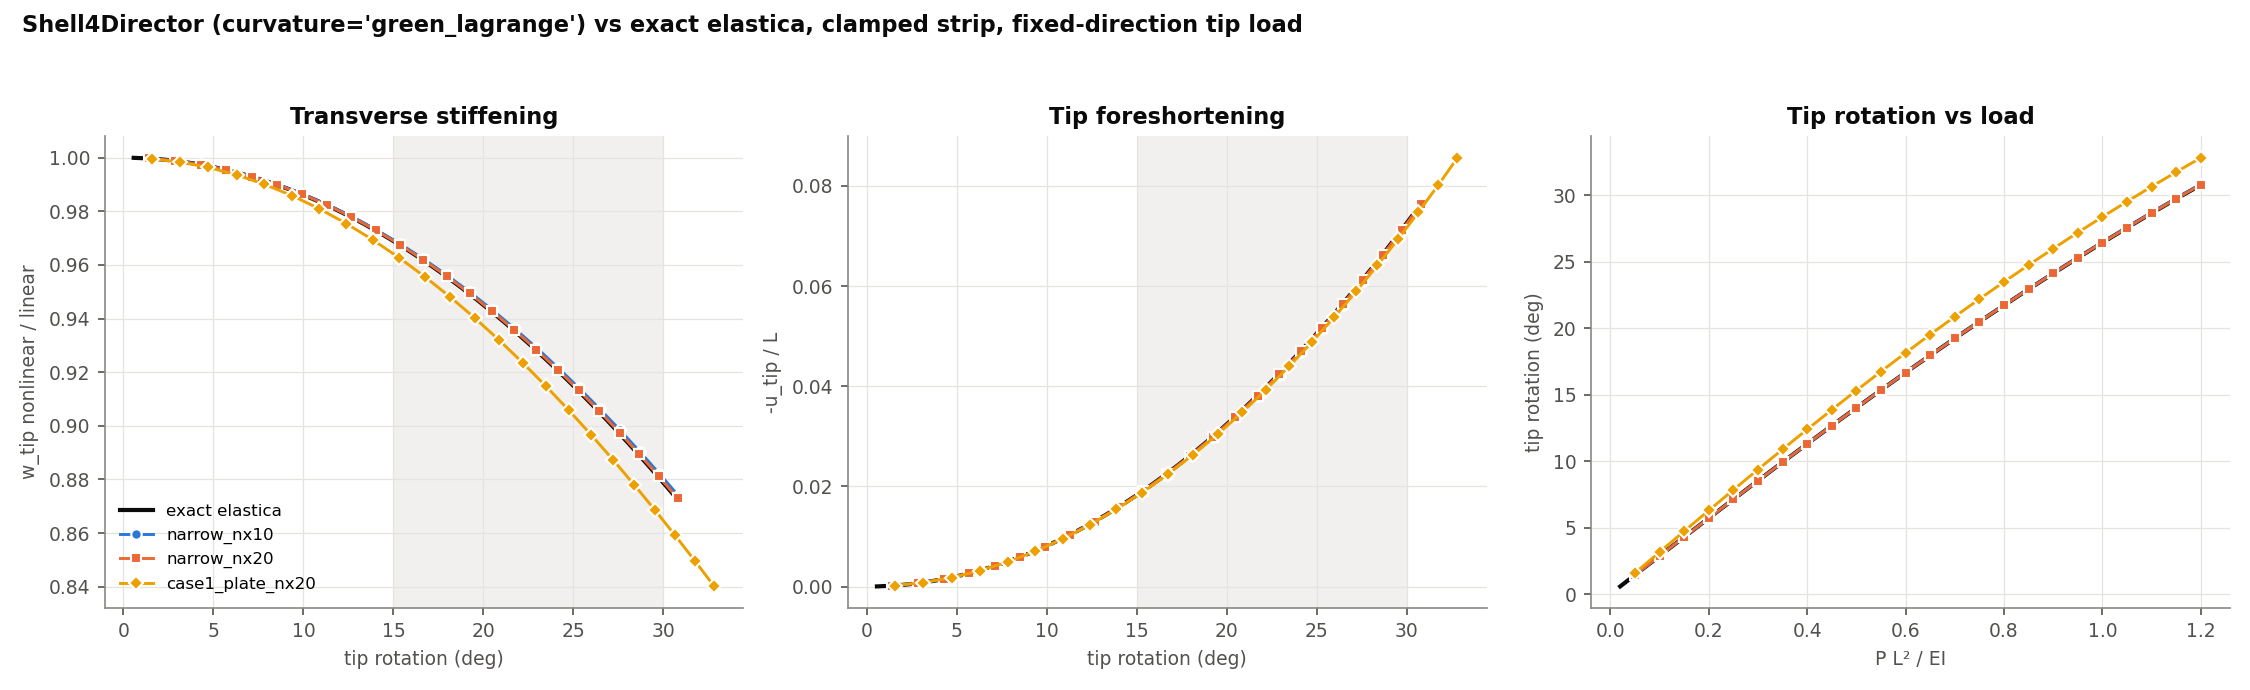
\includegraphics[width=0.8\linewidth]{figures/ch14r/hy_elastica.png}
\caption{Element check on a clamped strip against the exact elastica, for strips of increasing width and mesh density.}\label{fig:vf-hy-elastica}
\end{figure}

\subsection*{Results: case 1, plate with hole}

\emph{Full-order transient.} Over 200 steps of $\Delta t=0.005$~s the nonlinear response differs from the linear one by $12.8\,\%$ of the peak and the gap grows over the cycles, the signature of the publication's Fig.~6: the peak is $0.1910$~m nonlinear against $0.1969$~m linear (hardening). The publication reports roughly $20$--$40\,\%$ locally, so the magnitude is smaller here; the coarser mesh is a candidate cause that was not investigated.

\begin{figure}[tbp]
\centering
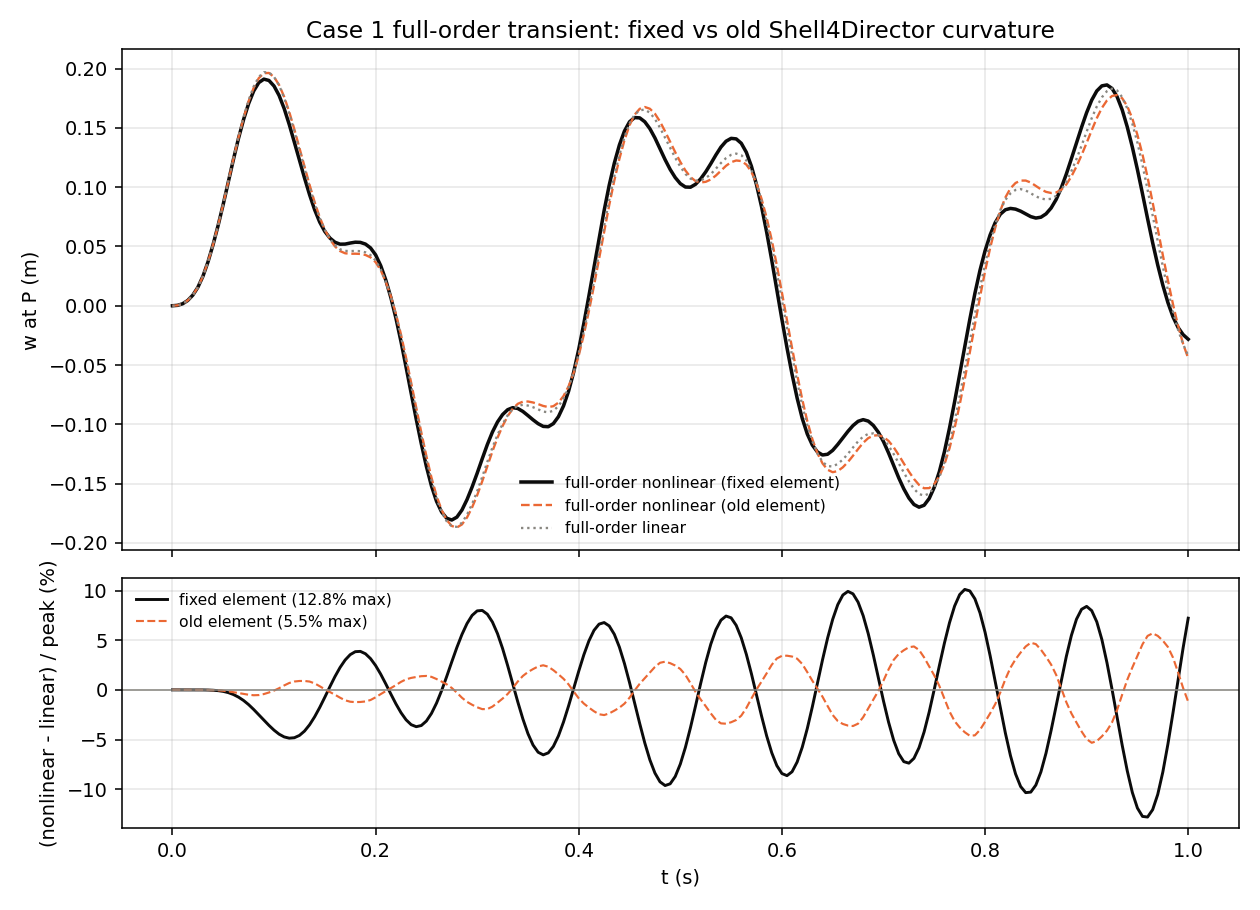
\includegraphics[width=0.8\linewidth]{figures/ch14r/hy_c1_fom.png}
\caption{Case 1: full-order transient, nonlinear (Green--Lagrange curvature) against linear.}\label{fig:vf-hy-c1fom}
\end{figure}

\emph{Static training and ROM transient.} The cubic fit of the 15 signed samples has a maximum training error of $0.71\,\%$; the static hardening in $q_1$ is $0.998$ (nonlinear over linear) at $q_1=0.05$ and $0.951$ at $q_1=0.25$. An earlier one-sided training range ($q_1\in[0.004,0.020]$) needed a tenfold extrapolation and gave $20\,\%$ error, which, and not the integrator, was the cause (\texttt{fixed\_point} and \texttt{newton} agree). \Cref{tab:vf-hy-c1} gives the transient errors.

\begin{table}[tbp]
\centering\footnotesize
\caption{Case 1: error of the transient against the full-order model.}\label{tab:vf-hy-c1}
\begin{tabular}{@{}lrr@{}}
\toprule
Model & Max error / peak & RMS error (m)\\
\midrule
Signed static fit, Newton (\texttt{fixed\_point}, $n=4$, identical) & $10.38\,\%$ & $7.99\times10^{-3}$\\
Linear modal ROM ($\mathbf F_{\rm nl}=\mathbf 0$) & $12.61\,\%$ & $1.07\times10^{-2}$\\
Linear full-order model & $12.81\,\%$ & $1.08\times10^{-2}$\\
\bottomrule
\end{tabular}
\end{table}

The nonlinear ROM beats the linear one only slightly: the linear ROM lags the full-order response and the nonlinear one leads it by a similar amount.

\begin{figure}[tbp]
\centering
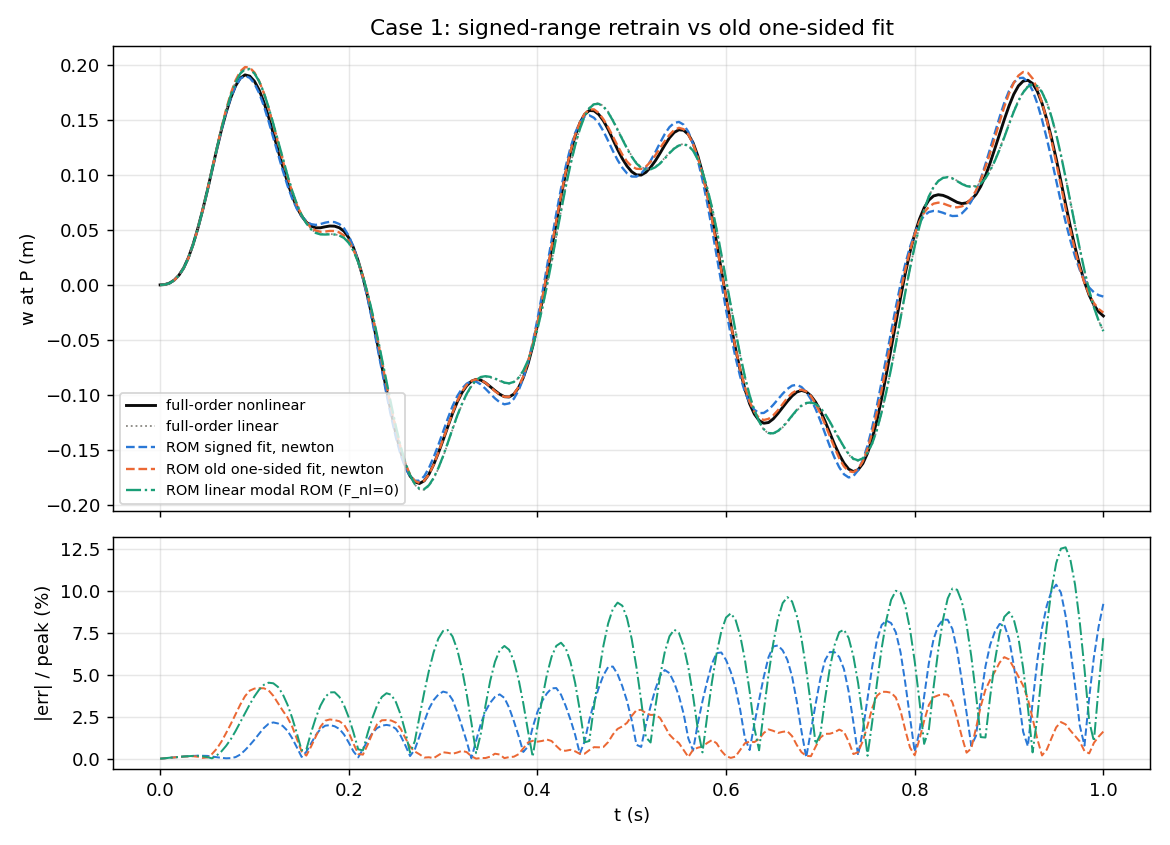
\includegraphics[width=0.8\linewidth]{figures/ch14r/hy_c1_rom.png}
\caption{Case 1: ROM transients against the full-order model. The one-sided earlier fit (trained on the faulty element) agrees only by accident and is not a better model.}\label{fig:vf-hy-c1rom}
\end{figure}

\emph{Backbone.} \Cref{tab:vf-hy-c1back} and \Cref{fig:vf-hy-backbone} show why: the ROM's static solve reproduces the full-order release state to about five digits, yet in free vibration the ROM's frequency shift is $4.7$ to $4.9$ times that of the full-order model. The full-order model retains only about $20\,\%$ of its static hardening in free vibration, because when a cantilever bends its tip moves inward and the inertia of that in-plane motion softens the response; a model trained on static solves contains no in-plane inertia and keeps all of the hardening. This also explains the ranking of \Cref{tab:vf-hy-c1}: the 2.5~Hz forcing is well below the 8.35~Hz mode, so much of the response is quasi-static, where the ROM is right and the linear ROM wrong, while the free-vibration part is where the ROM runs ahead. The report records this as an open defect; the option it recommends is to restore in-plane inertia through the membrane expansion of \rom{}, a change that needs sign-off, and the backbone test is the acceptance check of any fix.

\begin{table}[tbp]
\centering\footnotesize
\caption{Case 1: frequency shift in free vibration released from the static state $q_1$.}\label{tab:vf-hy-c1back}
\begin{tabular}{@{}rrrr@{}}
\toprule
Release $q_1$ & FOM shift & ROM shift & ROM / FOM\\
\midrule
0.05 & $+0.016\,\%$ & $+0.074\,\%$ & 4.7\\
0.10 & $+0.061\,\%$ & $+0.292\,\%$ & 4.8\\
0.15 & $+0.134\,\%$ & $+0.641\,\%$ & 4.8\\
0.20 & $+0.227\,\%$ & $+1.104\,\%$ & 4.9\\
0.25 & $+0.336\,\%$ & $+1.659\,\%$ & 4.9\\
\bottomrule
\end{tabular}
\end{table}

\begin{figure}[tbp]
\centering
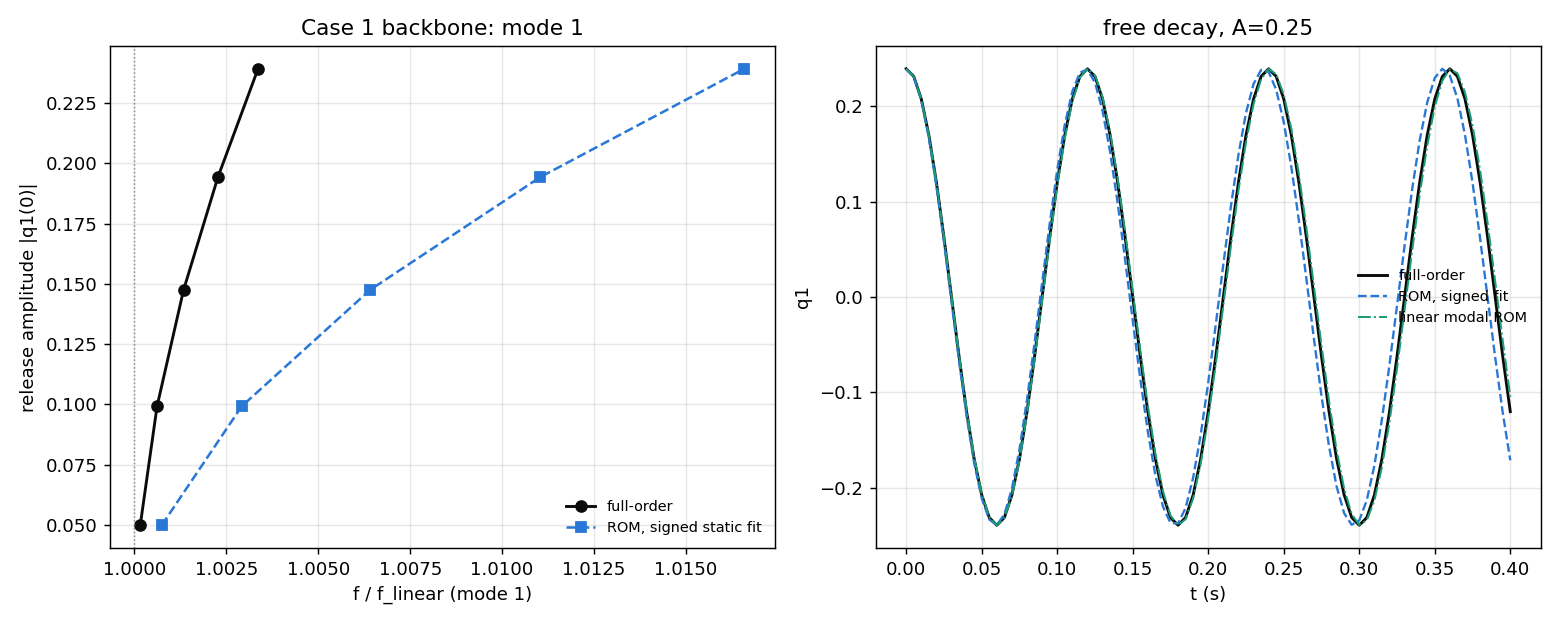
\includegraphics[width=0.8\linewidth]{figures/ch14r/hy_c1_backbone.png}
\caption{Case 1: backbone check. The ROM over-hardens and its phase runs ahead of the full-order model, while the linear ROM tracks it.}\label{fig:vf-hy-backbone}
\end{figure}

\subsection*{Results: case 2, cylindrical panel}

\emph{Static response.} The arc-length full-order solution (30 steps to 31.5~kN) shows a response that softens (tangent stiffness from 446 to about 240~N/mm by 2.5--3.5~kN, crown $w\approx8$--$12$~mm) and then hardens (about 2250~N/mm at 30~kN), matching the publication's softening below about 5000~N (\Cref{fig:vf-hy-c2static}). Ten single-branch Koiter--Newton points between 200~N and 10~kN lie on the curve to $\le10^{-5}$ relative above 600~N ($9\times10^{-4}$ at 200~N, where the interpolated reference is least accurate). The crown displacement is $7.69$~mm at 2.5~kN, $15.69$~mm at 5~kN and $22.46$~mm at 10~kN.

\begin{figure}[tbp]
\centering
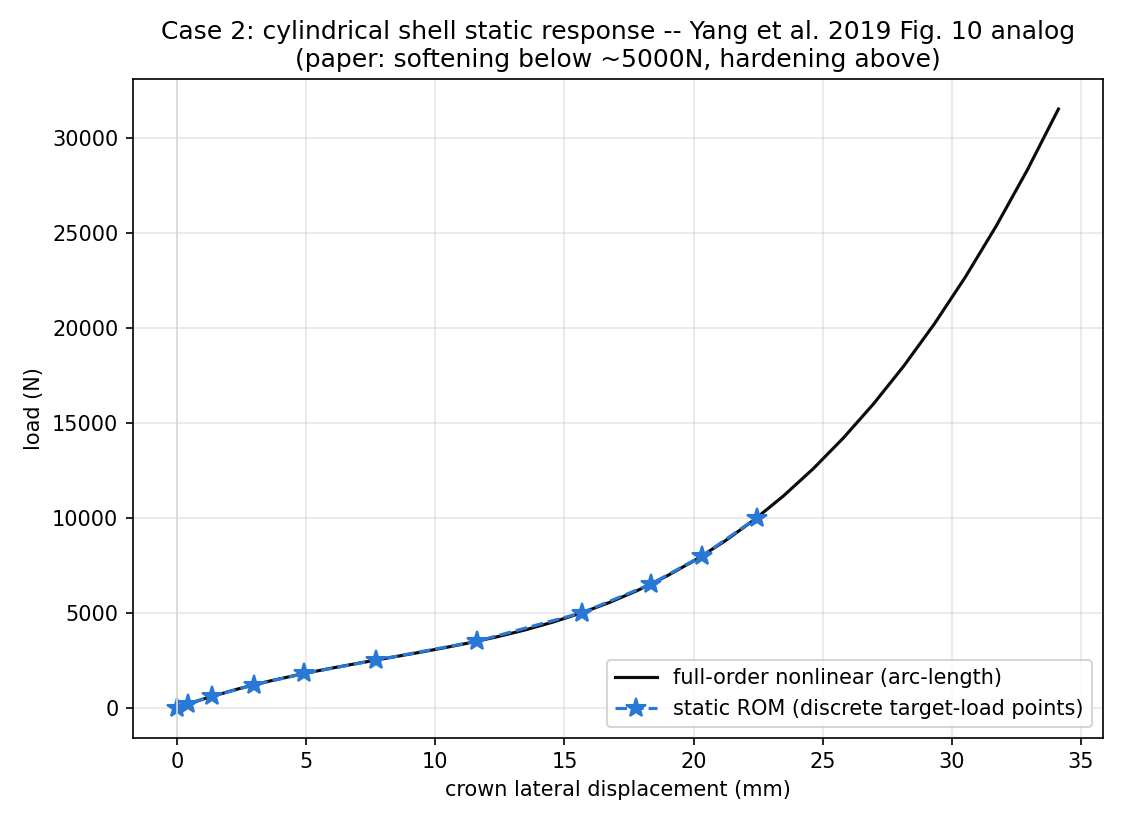
\includegraphics[width=0.7\linewidth]{figures/ch14r/hy_c2_static.png}
\caption{Case 2: static crown response, arc-length full-order solution (line) and Koiter--Newton points (stars).}\label{fig:vf-hy-c2static}
\end{figure}

\emph{Training fit.} Signed per-mode ranges, as fractions of the thickness, are $[-2.2,+2.5]$ for mode~1 and $\pm0.12$, $0.10$, $0.03$, $0.01$, $0.01$ for modes 6, 5, 9, 17, 16. All solves used Koiter--Newton with no fallbacks. \Cref{tab:vf-hy-fit} gives the fit error by mode set.

\begin{table}[tbp]
\centering\footnotesize
\caption{Case 2: training fit by mode set.}\label{tab:vf-hy-fit}
\begin{tabular}{@{}llrr@{}}
\toprule
Set & Modes & Samples & Max relative fit error\\
\midrule
2modes\_top & 1, 6 & 15 & $1.08\,\%$\\
2modes\_alt & 1, 5 & 15 & $0.76\,\%$\\
3modes & 1, 6, 5 & 21 & $0.32\,\%$\\
4modes & 1, 6, 5, 9 & 39 & $0.48\,\%$\\
6modes & 1, 6, 5, 9, 17, 16 & 101 & $1.61\,\%$\\
\bottomrule
\end{tabular}
\end{table}

\emph{Transient.} The full-order crown displacement spans $-12.1$ to $+23.0$~mm against $-16.6$ to $+16.1$~mm for the linear model, so the linear model is off by $70.6\,\%$ of the peak and every ROM here corrects a strongly nonlinear response (\Cref{fig:vf-hy-c2rom}, \Cref{tab:vf-hy-c2}). Two observations follow. Adding modes beyond three does not reduce the ROM error although the truncation floor keeps falling, so the remaining error is fit scatter and not truncation; and retraining over a wider range barely changed the errors, so the $3\,\%$ level is not extrapolation. A diagnostic on the six-mode model recovered the true nonlinear modal force along the transient and compared it with the fit: mode~1's fitted force matches it to $0.65\,\%$ at most ($0.26\,\%$ RMS) over the whole 5000~N transient even though $F_{\rm nl}$ reaches $63\,\%$ of the linear force; correcting mode~1 alone takes the error from $3.13\,\%$ to $1.62\,\%$, mode~6 alone to $2.42\,\%$, mode~5 alone to $2.66\,\%$; adding $q_1^4$ and $q_1^5$ terms does not help ($3.13\,\%$ to $3.13\,\%$), so the polynomial form is not the limit. Fit scatter of $0.3$--$1\,\%$ RMS is amplified about fivefold by the response, an accepted property of the method.

\begin{table}[tbp]
\centering\footnotesize
\caption{Case 2: transient error ($\varepsilon$ of \cref{eq:hy-err}) and the projection floor.}\label{tab:vf-hy-c2}
\begin{tabular}{@{}lrr@{}}
\toprule
Mode set & ROM (\texttt{newton} = \texttt{fixed\_point}) & Projection baseline\\
\midrule
2modes\_top & $6.51\,\%$ & $4.40\,\%$\\
2modes\_alt & $5.35\,\%$ & $5.03\,\%$\\
3modes & $2.83\,\%$ & $1.39\,\%$\\
4modes & $3.68\,\%$ & $0.71\,\%$\\
6modes & $3.13\,\%$ & $0.36\,\%$\\
\bottomrule
\end{tabular}
\end{table}

\begin{figure}[tbp]
\centering
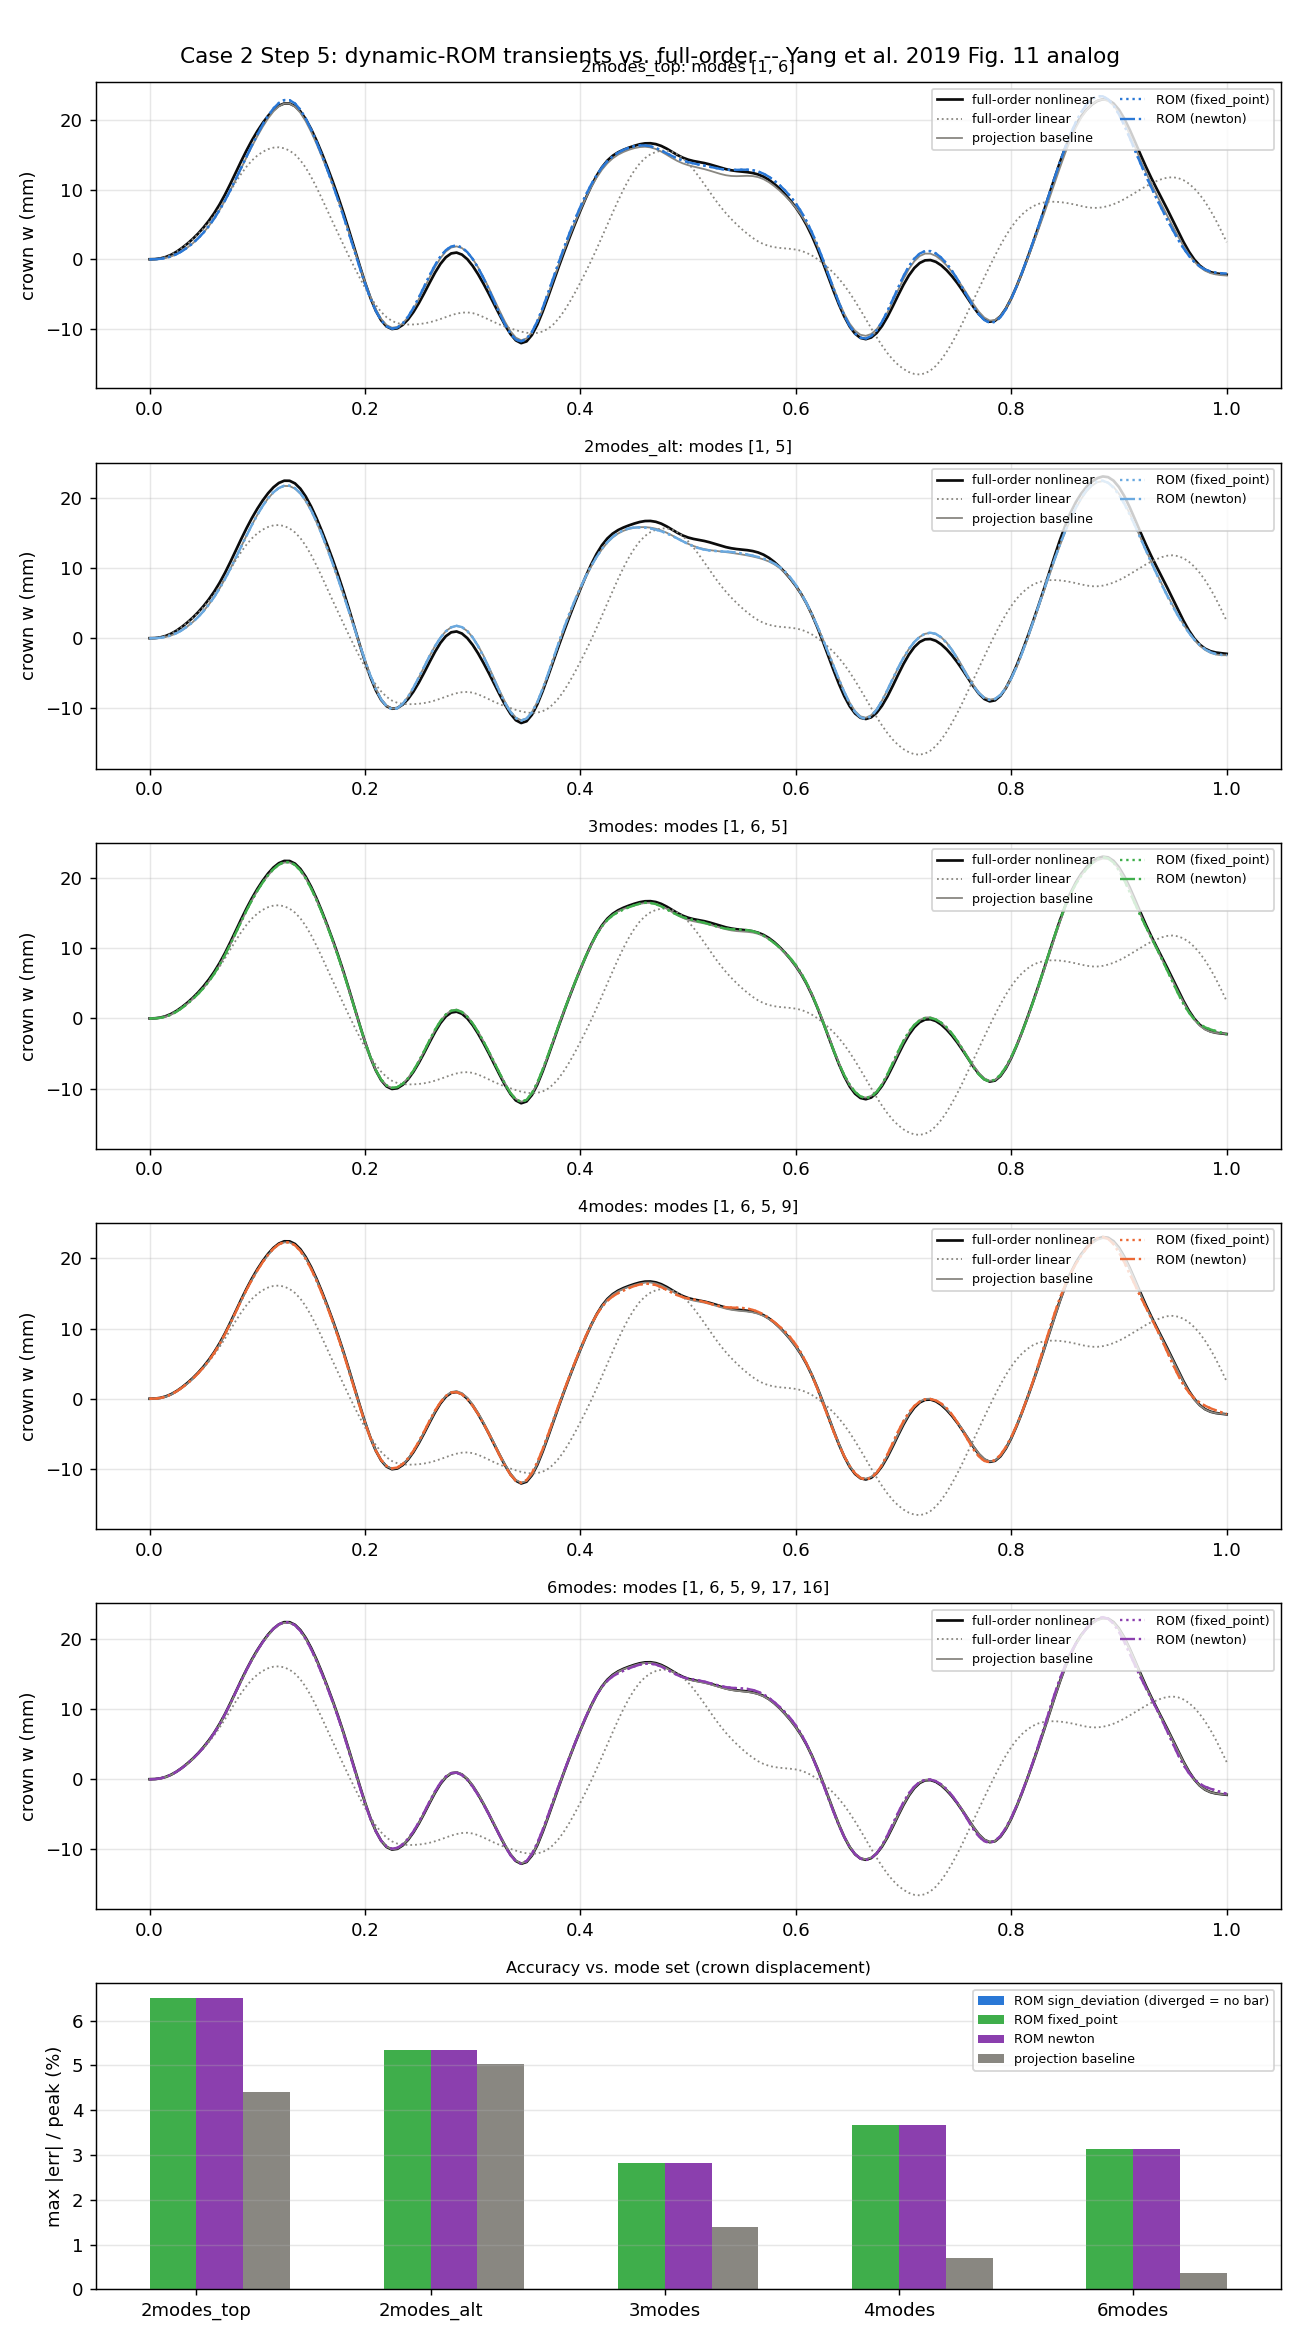
\includegraphics[width=0.75\linewidth]{figures/ch14r/hy_c2_rom.png}
\caption{Case 2: ROM transients for the five mode sets against the full-order crown displacement.}\label{fig:vf-hy-c2rom}
\end{figure}

\emph{Backbone.} Released from ten static states (push-in and pull-out), the orbits cross both sides. \Cref{tab:vf-hy-c2back} gives selected rows: the backbone first softens to $0.962$ and then hardens to $+12\,\%$; the six-mode ROM tracks it to within $0.09\,\%$ at all ten amplitudes and the two-mode ROM to within $0.5\,\%$, even on the two largest orbits, which slightly exceed the training range. The contrast with case~1 is the structure: here the nonlinearity is membrane stretching against fixed edges with no free in-plane motion, so static training captures the dynamics; in case~1 the free edge lets in-plane inertia matter and it does not.

\begin{table}[tbp]
\centering\footnotesize
\caption{Case 2: backbone $f/f_{\rm lin}$ by orbit half-range of $q_1$ (selected rows).}\label{tab:vf-hy-c2back}
\begin{tabular}{@{}rrrr@{}}
\toprule
Half-range $q_1$ & FOM & 6-mode ROM & 2-mode ROM\\
\midrule
2.4 & 0.9859 & 0.9857 & 0.9855\\
5.2 & 0.9624 & 0.9616 & 0.9603\\
6.9 & 0.9706 & 0.9697 & 0.9680\\
9.0 & 1.0209 & 1.0203 & 1.0201\\
10.4 & 1.0775 & 1.0782 & 1.0811\\
11.4 & 1.1197 & 1.1197 & 1.1250\\
\bottomrule
\end{tabular}
\end{table}

\begin{figure}[tbp]
\centering
\includegraphics[width=0.98\linewidth]{figures/ch14_hyrom.pdf}
\caption{Free-vibration check of the hybrid ROM of \citet{yang2019hybrid}: frequency relative to the linear one, full-order model against ROM. (a) Cylindrical panel: the ROM follows the softening and hardening, with a largest frequency error of \cvfHyPanelBack. (b) Plate with a hole: the ROM hardens about \cvfHyPlateRatio{} times too much at the largest amplitude.}\label{fig:vf-hyrom}
\end{figure}

\subsection*{Solver changes the study required}

Six changes to the solver stack were needed to reproduce these results and affect trust in the numbers. (1) \texttt{Shell4MITC}: the two shear rows used the same sign convention, which is wrong for a rotation vector; the defect was invisible on axis-aligned meshes and gave frequencies 3 to 10 times too high on meshes with differently oriented elements (the circular hole), and was found by relabelling the nodes of an element cyclically (the stiffness must be invariant under permutation). (2) \texttt{Shell4Director}: curvature from the moderate to the Green--Lagrange measure. (3) Koiter--Newton: a frozen-tangent chord corrector diverged on a truly nonlinear element. (4) Koiter--Newton: an absolute $10^{-4}$ finite-difference probe was swamped by roundoff at coordinates near 2540~mm and was replaced by a scale-aware probe (default relative step $10^{-2}$). (5) The generic $m=1$ Koiter--Newton driver had a false detection (a trace-based threshold inflated by membrane stiffness) and a corrector that could not move; both were fixed with regression tests. (6) The default integrator of \rom{} changed from \texttt{sign\_deviation} to \texttt{fixed\_point}.

\subsection*{Comparison with the publication}

\begin{table}[tbp]
\centering\footnotesize
\caption{Outcome of the reproduction of \citet{yang2019hybrid}.}\label{tab:vf-hy-cmp}
\begin{tabularx}{\linewidth}{@{}>{\raggedright\arraybackslash}p{3.8cm} >{\raggedright\arraybackslash}X >{\raggedright\arraybackslash}p{2.4cm}@{}}
\toprule
Quantity & This work & Outcome\\
\midrule
Case 1 modes (Table~1) & within $0.3$, $0.9$, $2.8$, $2.9\,\%$; 1224 against 2394 dofs & reproduced\\
Case 1 full-order transient (Fig.~6) & $12.8\,\%$ gap, hardening (publication $\approx20$--$40\,\%$) & partly\\
Case 1 ROM transient & $10.4\,\%$ against $12.6\,\%$ for a linear ROM & partly\\
Case 1 free vibration & ROM over-hardens $4.7$--$4.9\times$ & not reproduced (open defect)\\
Case 2 static response (Fig.~10) & softening then hardening; points on the curve to $\le10^{-5}$ & reproduced\\
Case 2 ROM transient (Fig.~11) & $2.8$--$6.5\,\%$ against a $70.6\,\%$ linear gap & reproduced\\
Case 2 free vibration & within $0.09\,\%$ (6 modes) & reproduced\\
\bottomrule
\end{tabularx}
\end{table}

\subsection*{Departures from the publication's set-up}

The case-1 mesh has 1224 degrees of freedom against the publication's 2394. The training design is optimal Latin hypercube sampling and not the publication's combinatorial grid (its Eqs.~10--14). Case~1's final retraining uses incremental Newton because Koiter--Newton stalls at those amplitudes; case~2 uses Koiter--Newton at discrete target loads and not $m=1$ continuation. The case-2 load is spread over a $3\times3$ patch, and its modes are chosen by load projection, not by hand. The publication's \texttt{sign\_deviation} integrator diverges and is excluded. The remaining limits are the case-1 over-hardening (defect D6), the $12.8\,\%$ against $20$--$40\,\%$ full-order gap, an error floor near $3\,\%$ for three or more modes of case~2, and the lack of an independent reference for the publication's absolute numbers: its figures were compared by reading, not digitising. The main pipeline script of case~1 last ran with the old element and one-sided training, so its outputs are stale and superseded by the standalone scripts; folding the signed training into it and re-running (two hours or more) has not been done. Mode-shape signs depend on the BLAS thread count, so modal quantities are built once in the parent process.
